%   MSc Business Analytics Dissertation
%
%   Title:     Literature Review
%   Author: Conor Reid
%
%   Chapter 3: Literature Review
%
\chapter{Literature Review}\label{C.LitReview}
\section{Introduction}\label{S.intro3}
{This literature review first presents some of the ways that corporate success can be quantified. This includes how it is defined by \cite{moldovan2015learning}, as well as by others whose approaches may benefit this study. This is followed by an analysis of literature pertaining to the relationship between corporate governance and company performance, again including the work of \cite{moldovan2015learning} as well as other relevant studies. This review finishes with an exploration of literature regarding causation and the statistical techniques used to infer causation. There is also discussion on the issues that arise in attempting to do so, and how they can be addressed. }
\section{Company Performance - Measures and Factors}
{Among the key aspects of this study is the quantifying of corporate success, in a way that accurately   represents good and bad corporate performance. There are many aspects to this. For example, many different financial ratios have been developed that attempted to assign numerical performance ratings to companies taking into account a variety of accounting indictors. \cite {eidleman1995z} states that these ratios are often created by academics, and outlined the patterns they tend follow. He desribes how researchers find a sample of companies that meet some predetermined criterion of failure, as well as another sample of comparable firms (size, industry etc) that differ only in financial health. Common statistical learning can then be used to analyse which ratios can accurately separate the groups. Those which do so are kept, the rest discarded. Weights are assigned to each ratio to reach an aggregate equation. New firms are scored, and real-world performance recorded to measure how useful the new ratios are. \\\\
Blindly following financial ratios is often suboptimal and can be thought of as an over-reliance on simple stock price indicators. Perhaps the inclusion of more varied and diverse measures are required, such as the companies social responsibility commitments, and their impact on the environment. Both may contribute to a more accurate picture of corporate performance, and are discussed below.       }
\subsection{Financial Ratios}
{One of the indicators of corporate performance used by \cite{moldovan2015learning} is Tobin's Q score. This measure was devised by \cite{tobin1969general} who postulated that the combined market value of a given company should be equal to their replacement costs. This is described as the ideal state, with any deviation either way (a ratio above or below 1) warranting investment or the selling of assets. The use of this measure is well established in the literature, by \cite{chung1994simple}, 
\cite{bhagat2008corporate} and \cite{bolton2011unified}. \cite{chung1994simple} state that Tobin's Q plays an important part in financial interactions, and is employed to explain diverse corporate phenomena during the decision making process. \cite{bolton2011unified} used Tobin's Q to propose a model for dynamic investment and risk management and found that investment is best driven by the Q score as well as to the marginal value of liquidity.\\\\
The formal definition of Tobin's Q is given by \cite{chung1994simple} as; 
\begin {equation}\label{TobinQ}
L-R  \quad q = \small {\frac{PREFST + VCOMS + LTDEBT + STDEBT - ADJ}{TOTASST - BKCAP + NETCAP}}
\end{equation}\\
There is debate as to the practically of the Q score. \cite{chung1994simple} go on to state that the Q score is often neglected in real-world situations. One of the reasons they give for this is the complexity of the necessary calculations, and a potential unfamiliarity with its operational intricacies. Another reason is the unavailability of relevant data, particularly with high accuracy and in real-time. To counteract this, they worked to create and test an accurate approximation of Tobin's Q that utilises only basic financial information. They conclude that their approximation is close enough to the more formal definition to be used where more exhaustive calculations are not possible. \\\\
\cite {dybvig2010tobin} criticise Tobin's Q more strongly, stating that it is fundamentally malformed as a measure of corporate performance. They highlight long-serving managers as risk adverse, and who "...can {\it enjoy the quiet life} and underinvest". A logical implication of this is that firms invest less and operate well below their profit-generating capacity and thus reduces their net-present value. However, such is Tobin's Q formulated, underinvestment by a firm increases its Q score. They go on to explain the scores ambiguity, COME BACK TO. \\\\Another measure of corporate success used by \cite{moldovan2015learning} is the Altman Z score, which is often used as a probabilistic measure of whether a company will go into bankruptcy within the next two years. It can also be used more generally as a financial distress measure and to predict corporate defaults. The authors point out that there is much advocacy in the literature for using this measure, and this study was unable to find any that strongly reject its usefulness. The Altman Z score is given as;
\begin {equation}\label{AltmanZScore}
\begin{aligned}
Z \ Score \quad = \quad & 1.2\bigg(\frac{Working \ Capital}{Total \ Assets}\bigg) \ + \\\\
		& 1.4\bigg({\frac{Retained \ Earnings}{Total \ Assets}}\bigg) \ + \\\\
		& 3.3\bigg({\frac{Earnings \ before \ Interest \ and \ Tax}{Total \ Assets}}\bigg) \ + \\\\
		& 0.6\bigg({\frac{Market \ Value \ of \ Equity}{Total \ Liabilities}}\bigg) \ + \\\\
		& 1.0\bigg({\frac{Sales}{Total \ Assets}}\bigg)
\end{aligned}
\end{equation}\\
Among those that support this scores use is \cite {eidleman1995z}, who discusses its use in practice. He begins by highlighting Altman's own tests using the Z score which involved predicting 72\% of bankruptcies two years prior to the event, although the sample size or companies involved are not mentioned. Eidleman argues that the Z score is tried and tested, and;
\begin {quote}
It has been demonstrated to be quite reliable in a variety of contexts and countries. 

\hspace{2cm}---  \cite {eidleman1995z}
\end{quote}
Eidleman also outlines circumstances that warrant corrections and alterations to equation \ref{AltmanZScore}, in order to generalise it beyond its originally intended means. He argues that before being able to use the Z score, one must ensure the company in question is comparable to those involved in Altman's original study. Altman considered manufacturing and small firms in his original analysis, thus corrections must be made before scoring companies in different industries. Eidelman points to two specific circumstances here. \\\\
The first considers privately held companies, whose stocks are no publicly traded meaning term four of equation \ref{AltmanZScore} cannot be calculated. To correct for this, the Z score can be re-estimated using book values of equity. In other words, details from balance sheets published by private firms voluntarily can be used rather than details gleamed from the stock market. Certainly a work-around here is to consider solely publicly traded companies. A consequence of this is that such an analysis would only include companies that are bound by the the corporate governance code in their jurisdiction, which would need to be taken into account in studies such as this one.\\\\ Eidleman's second consideration is for non-manufacturing firms. The fifth term of equation \ref{AltmanZScore}, according to Eidleman, varies significantly by industry. He argues that merchandise firms for example, are significantly less capital intense and thus are much more likely to enjoy higher asset turnover and consequently Z-Scores. Z scores then would be likely to under-predict bankruptcy in these cases. In order to correct for this, a recommendation comes from Altman to eliminate the fifth term and adjust the weights. The adjusted equation \ref{AltmanZScoreAjusted} is shown below;
\begin {equation}\label{AltmanZScoreAjusted}
\begin{aligned}
Z \ Score \quad =  \quad & 6.56\bigg(\frac{Working \ Capital}{Total \ Assets}\bigg) \ + \\\\
		& 3.26\bigg({\frac{Retained \ Earnings}{Total \ Assets}}\bigg) \ + \\\\
		& 6.72\bigg({\frac{Earnings \ before \ Interest \ and \ Tax}{Total \ Assets}}\bigg) \ + \\\\
		& 1.05\bigg({\frac{Market \ Value \ of \ Equity}{Total \ Liabilities}}\bigg) \ \\\\ 
\end{aligned}
\end{equation}\\
Overall, the Altman Z score seems a highly appropriate indicator of corporate financial strength and thus success, and one that should be considered in this study. Consideration will need to be had for the type of industry included in this analysis, that will inform the exact calculation of the Z score itself. }
\subsection{Environmental Considerations}
{As mentioned previously, there is likely much room for improvement in quantifying corporate success beyond financial ratios. One potentially useful alternative is the link between environmental and economic performance, studied by \cite{schaltegger2002link}. The authors present two conflicting viewpoints in this space. The first states that improved environmental performance predominantly causes an increase in operating costs, which in turn negatively effects the profitability of the company. The second viewpoint states the opposite; improving a firms environmental performance in fact induces cost savings, which drives increases in profitability. These viewpoints are visualised in figure \ref{ch3_successAndEnviornment}. 
\begin{figure}[h] 
\centering
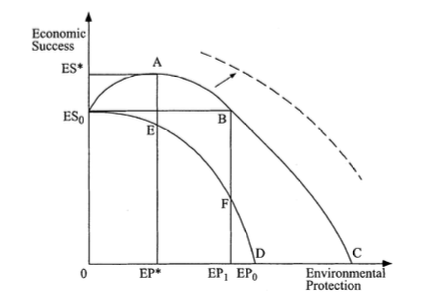
\includegraphics[scale = 0.7]{images/ch3_successAndEnviornment.png}
\caption{Potential correlations between corporate environmental protection and economic success.}
\label{ch3_successAndEnviornment}
\end{figure}\\
$ES_0$ represents the current level of economic success (this is described as a certain shareholder value), which decreases as spending in environmental protection increases (through points E and F, to D where non profit can be made). This is the pessimistic view, or the expectation that spending in this space reduces profit making ability to eventual zero. The more optimistic view is represented by the path from $ES_0$ through points A and B to point C (again where no profit is possible). This represents the ideology that some economic gain can be achieved, at least to some degree before tailing off, by being environmentally conscious. \\\\
The authors draw two conclusions from figure \ref{ch3_successAndEnviornment}. First, they argue that environmental performance can vary at a given level of economic success. Secondly, the reverse; that economic success can vary for a given level of environmental protection. These are key points, since it indicates that the former may not be a good predictor for the latter, and that an uplift in economic success is not guaranteed with increased environmental efforts. The authors conclude that the correlation between economic and environmental performance depends on not just company externalities but internal variables which are influenced by management. It is firm management, who moderate this relationship, that must be optimised in order to gain economically. The authors put this forward as an explanatory variable not considered in the literature to this point. \\\\It is natural then to ask how this can be realised in analysis. \cite{schaltegger2002link} suggest two cases from which data may be derived. The first relates to the firms ability to utilise to the full the economic benefits of environmental protection measures. This may materialise in R\&D spending, or other marketing positioning that communicates their efforts and establishes them as industry leaders. The second relates to how this reputation is achieved in practice, by realising the optimal environmental performance for maximum economic success. This can take the form of identifying the most optimal way to reach clean production for example.\\\\
\cite{wahba2008does} also perform research in this area, studying whether the market values corporate environmental responsibility, specifically in an Egyptian context. Similarly to \cite{schaltegger2002link}, the authors acknowledge divided and inconclusive literature on this topic, stating an aim to present empirical evidence on how engagement with environmental responsibility can influence corporate market value. For their analysis they looked at a sample of 156 firms across 19 industries, using firm market value as the dependant variable (interestingly, quantified by Tobin's Q score mentioned previously). Important to note is the authors use of ISO 14000/14001 certification as a proxy for environmental performance. This is recognised by the authors as non-ideal, however this may still have some utility in future research to address the difficulty in quantifying performance in this area. \\\\ \cite{wahba2008does} state that the overall finding of this research is that the market does in fact reward firms for their environmental efforts, by positively influencing that firms Tobin's Q score, but do point to similar issues raised by \cite{schaltegger2002link}. Namely, that a companies decision to reduce their impact on the environment comes with significant cost and that if this is not managed correctly, the economic benefits evaporate.     \\\\
There is clear support in the literature for the presence of a relationship between corporate economic success and environmental performance. \cite{schaltegger2002link} suggest it is the firm management of environmental considerations that influences success, and put this forward as an explanatory variable not yet considered in literature. This theory is supported by \cite{wahba2008does}, who find a strong relationship in this space but with a caveat that management plays a significant role in realising benefits. It remains to be seen exactly how this can be realised in data analysis. }
\subsection{Corporate Social Responsibility}
{Corporate social responsibility, or CSR, is defined by the European Commission as "the responsibility of enterprises for their impacts on society". This is similar to being conscious of environmental impact, but can be generalised to include compliance with established ethical standards and national and international norms. Central to CSR is the creation of shared value between themselves and their stakeholders and the larger society as well as mitigating their possible adverse impacts with those groups. It is natural to consider elements of CSR then, when discussing firm success metrics. \\\\
\cite{orlitzky2003corporate} begin their research in this space by stating 
\begin{quote}
Most theorizing on the relationship between corporate social / environmental performance (CSP) and corporate financial performance (CFP) assumes that the current evidence is too fractured or too variable to draw any generalizable conclusions.

\hspace{2cm}--- \cite{orlitzky2003corporate}
\end{quote}
Their research aims to show this claim is unfounded, and provide a more rigorous methodology for drawing such conclusions. They argue that many authors have attempted to find causal relationships between CSP and CSR, but have failed in part due to a failure to see vital differences between theory and operational applications. They also state that an aim of their research is to aggregate knowledge in the area, and highlight important findings they believe to be overlooked. Meta-analysis have been proven to proved value where a number of disparate and conflicting results mean the field is inconclusive.\\\\
They present a number of hypotheses. They first states that CSP and CFP are positively related, regardless of industry and the context of the given study relating the two. They base this on a number of studies, stating that CSP is a vital form of "good management theory" that boasts competitive advantage by addressing stakeholder concerns quickly and fairly.  Secondly, they hypothesise on the temporal nature of this relationship. They state that there is a bidirectional causality between CSR and CFP. That is, there is a circular casual relationship that governs performance in each area. This is supported by the idea that prior success in CFP facilitates positive engagement in CSP, due to increased responsibility and freedom at the managerial level. \\\\
The third hypothesis put forward by \cite{orlitzky2003corporate} involves the underlying logic behind the correlation between CSP and CFP. The first is that CSP boasts managerial competencies and organisational efficiency, by enabling shared knowledge of the firm's market as well as social and political environments. Secondly they suggest that CSP is a driving factor behind the firm's reputation, and thus elicits significant goodwill from stakeholders. The fourth and final hypothesis put forward involves the methodology used by previous studies to draw conclusions from. The authors here suggest that the variance in results seen across studies can be explained by sampling or measurement error, for example. 
\\\\
In order to support these claims, \cite{orlitzky2003corporate} perform a meta-analysis involving 52 studies across both CSP and CFP, resulting in a total sample size of 33,878 observations on which they perform their analysis. This analysis involves a statistical aggregation technique to be applied, which calculated the cumulative correlations across studies, correcting for variable elements of those studies to reach one "true score correlation ($\rho$)". Using this technique, the authors were able to explain 24\% of the cross-study variance in relation to the observed r value, which they suggest is significant. That is, by controlling for sampling and measurement errors across multiple studies, they could reduce the variation in results by 25\%. They suggest that this, strengthened with other analysis, supports their first hypothesis. 


}
\section{Corporate Governance and Company Performance}
\subsection{Governance Models}
\subsection{Influence of Governance on Performance}
\section{Inferring Causation}
\subsection{Introduction}
\subsection{Techniques}
\subsection{Examples}